\documentclass[12pt,twocolumn]{article}
\usepackage[brazil]{babel}
\usepackage[utf8]{inputenc}
\usepackage{graphicx,color}
\usepackage{amsthm,amsfonts}
\setlength{\textwidth}{17 cm}
\setlength{\textheight}{20 cm}
\evensidemargin 0 cm
\oddsidemargin 0 cm
\setlength\parskip{4 pt} 
\title{Problema da Cobertura}
\author{Nilton Flávio Sousa Seixas}


\begin{document}
\maketitle{}
\tableofcontents
\begin{abstract}
O resumo do resumo.
\end{abstract}
\begin{abstract}
O resumo do resumo.
\end{abstract}
\begin{figure}[!thb]
\centering
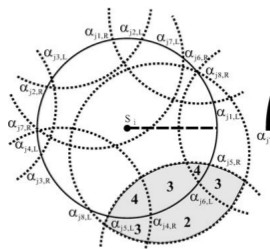
\includegraphics[scale=0.5]{teste.jpg}
\caption{Legenda}
\label{Rotulo}
\end{figure}
\section{Candy shop}
bla bla bla
\section {super freak}



	
\end{document}
